Второй отборочный тур делится на 3 этапа. Победители определяются по сумме победных очков за все три этапа. Одновременно доступен только один из этапов. После окончания текущего этапа и начала следующего, внутренние баллы сбрасываются и меняется цель, вернуться к задачам из предыдущего этапа невозможно.

\textit{Этапы:}
\begin{enumerate}
    \item[1 Этап.] 20 дней – Производство дисплеев. Участникам предстоит синтезировать квантовые точки трех цветов – красного, зеленого и синего, после чего – изготавливать на их основе дисплеи.
    \item[2 Этап.] 14 дней – Производство солнечных батарей. Участникам предстоит синтезировать квантовые точки, позволяющие эффективно поглощать солнечное излучение. Затем участники создают солнечную батарею, работающую на полученных квантовых точках.
    \item[3 Этап.] 14 дней – Производство биометок. Участники синтезируют квантовые точки, которые возможно детектировать в организме человека, после чего формируют антитела для связи с наночастицами, и, наконец, создают биометки.
\end{enumerate}

Вначале каждого этапа команда получает фиксированный стартовый объем денег – 500 000 \textpeso. Деньги тратятся на
\begin{itemize}
    \item компьютерное моделирование конечного продукта, где участники понимают какие параметры наночастиц требуются для создания наиболее качественного целевого продукта (10 000 \textpeso / попытка);
    \item проведение лабораторных испытаний - синтеза наночастиц под конечную цель (10 000 \textpeso / попытка);
    \item исследование параметров полученных квантовых точек: определение длины волны люминесценции (стоимость 1000 \textpeso), квантового выхода люминесценции (стоимость 1000 \textpeso), состава (стоимость 1000 \textpeso), стабильности (стоимость 3500 \textpeso) и токсичности квантовых точек (стоимость 4500 \textpeso);
    \item изготовление конечного продукта (стоимость партии дисплеев – 100 000 \textpeso, солнечной батареи – 100 000 \textpeso и биометок – 100 000 \textpeso).
\end{itemize}

После успешного синтеза наночастиц есть возможность, проведя необходимые лабораторные исследования получить инвестиции (добавку денег). Так на Этапе 1, для инвестора важна точность попадания в длину волны люминесценции наночастиц (чистота цвета), а также квантовый выход наночастиц. На Этапе 2 становится важнее стабильность, а квантовый выход – не важен На Этапе 3 – важны все параметры наночастиц: длина волны, квантовый выход, токсичность и стабильность. Формулы по рассчету количества дополнительных денег на каждом этапе приведены ниже:

Этап 1: $I (1)= \lambda_1\times Q\times 100 \: 000$ \textpeso (можно получить по 1 разу для каждого цвета наночастиц, максимум – 300 000 \textpeso, так как цвета 3 – красный, синий и зеленый)

Этап 2: $I (2)= \lambda_2\times Q\times 300 \: 000$ \textpeso

Этап 3: $I (3)= \lambda_3\times Q\times 300 \: 000$ \textpeso

Первый шаг на каждом этапе – проектирование (или моделирование) конечного дисплея, солнечной батареи или биометок, входе чего участники понимают какого параметра квантовые точки им требуются, на какие параметры следует обратить больше или меньше внимания при синтезе. В дальнейшем удовлетворение заданным параметрам напрямую влияет на параметр «качество» как квантовых точек, так и целевого продукта.

При этом выделяют продукт первого уровня (квантовые точки) и продукт второго уровня (итоговое устройство). Как следует из описания выше, участникам необходимо сначала «заглянуть» в продукт второго уровня, чтобы приступить к созданию продукта первого уровня, который, в свою очередь, позволит создать наиболее качественный продукт второго уровня.

Ниже приводится таблица, где указано какие параметры являются важными для продукта каждого уровня: 
\begin{table}[H]
	\begin{center}
		\begin{tabular}{|p{2cm}|p{3cm}|p{8cm}|}
			\hline
			Номер этапа	& Уровень продукта / название & Важные параметры \\
			\hline
			1 (дисплеи)	& 1 / квантовые точки с синей люминесценцией	& \begin{itemize}
				\item длина волны 460 \textpm 15 нм
				\item наибольший квантовый выход
				\item мmасса наночастиц
				\end{itemize} \\
				\hline
			1 (дисплеи)	& 1 / квантовые точки с зеленой люминесценцией	& \begin{itemize} \item длина волны 550 \textpm 15 нм
				\item наибольший квантовый выход
				\item масса наночастиц \end{itemize} \\
				\hline
			1 (дисплеи)	&1 / квантовые точки с красной люминесценцией		& \begin{itemize} \item длина волны 640 \textpm 15 нм
				\item наибольший квантовый выход
				\item масса наночастиц \end{itemize} \\
				\hline
			1 (дисплеи)	&2 / дисплей & \begin{itemize} \item длина волны люминесценции наночастиц трех цветов
				\item наибольшие квантовые выходы наночастиц
				\item наименьший разброс в квантовых выходах наночастиц
				\item толщина слоя наночастиц на дисплее \end{itemize} \\
				\hline
			2 (солнечные батареи)	& 1 / квантовые точки		& \begin{itemize} \item длина волны больше 600 нм
				 \item стабильность не менее 40\%
				 \item масса наночастиц \end{itemize} \\
				 \hline
			2 (солнечные батареи)	& 2 / солнечная батарея		& \begin{itemize} \item положение ширины запрещенной зоны позволяет эффективно разделять носители заряда
				\item толщина слоя наночастиц на батарее \end{itemize} \\
				\hline
			3 (биометки)	& 1 / квантовые точки		& \begin{itemize} \item длина волны в окне прозрачности крови
				\item минимальная токсичность
				\item максимальная стабильность
				\item высокий квантовый выход \end{itemize} \\
				\hline
			3 (биометки)	&2 / биометки		& \begin{itemize} \item конструкция антитела (состав вариабильных доменов и размер)
				\item определяют параметры наночастиц \end{itemize} \\
				\hline
		\end{tabular}
	\end{center}
\end{table}

Качество продуктов первого уровня на всех этапах
Перед проведением синтеза наночастиц, участники вводят целевые параметры квантовых точек: планируемый состав, длину волны излучения, квантовый выход, стабильность, токсичность и массу наночастиц согласно запросу продукта второго уровня. Формула для расчета качества итогового продукта первого уровня - квантовых точек, на всех этапах:
$$q_1 (1)=  \frac{\lambda+Q+s+\tau+m}{5},$$
где $\lambda$ – параметр длины волны наночастиц, который равняется 1, если длина волны попадает в заявленную длину волны с точностью \textpm 50 нм, и равен 0, если не попадает. $Q$ – параметр квантового выхода наночастиц, равен 1, если полученное значение квантового выхода не более чем на 10\% ниже заявленного вначале значения. s -стабильность квантовых точек, равна 1, если полученное значение стабильности не более чем на 10\% ниже заявленного вначале значения. Параметр $\tau$ – НЕтоксичность соединения, на основе которого получены наночастицы. Токсичность рассчитывалась по следующей таблице, $\tau$ рассчитывалась как (100\%-Токсичность, \%)/100\%:

\begin{table}[H]
	\begin{center}
		\begin{tabular}{|l|c|c|}
			\hline
			Соединение	&Токсичность, \% &$\tau$ \\
			\hline
			$CsPbCl3$	&40&0.6 \\
			\hline
			$CsPbBr3$	&40&	0.6 \\
			\hline
			$CsPbI3$	&40	&0.6 \\
			\hline
			$CdS$	&70	&0.3 \\
			\hline
			$CdSe$	&80	&0.2 \\
			\hline
			$CdTe$	&90	&0.1 \\
			\hline
			$PbS$	&50&	0.5 \\
			\hline
			$PbSe$	&60&	0.4 \\
			\hline
			$InP$	&40	&0.6 \\
			\hline
			$ZnSe$&	30&	0.7 \\
			\hline
			$CuInS2$&	25	&0.75 \\
			\hline
		\end{tabular}
	\end{center}
\end{table}

Синтез наночастиц заканчивался неудачей в случае, если параметр $\tau$ полученных частиц был более чем на 10\% ниже заявленного значения. $m$ – масса квантовых точек, должна быть нем менее чем на 2\% выше заявленного значения, в этом случае $m = 1$, иначе $m = 0$. Следует отметить, что равенство хотя бы одного параметра нулю приводило к неудачному синтезу и требовало осуществления новой попытки. При этом участникам (в зависимости от неудачи) писалось одно из следующих сообщений:

\begin{itemize}
	\item «Стабильность полученных частиц более чем на 10\% ниже заявленного значения»
	\item «Токсичность полученных частиц более чем на 10\% превышает заявленное значение»
	\item «Квантовый выход полученных частиц более чем на 10\% ниже заявленного значения»
	\item «Отклонение массы полученных частиц»
	\item «Отклонение длины волны люминесценции полученных частиц от запланированного значения превышает 50 нм»
\end{itemize}

Программная проверка велась в следующем порядке: стабильность, токсичность, квантовый выход, масса и длина волны. Т.е. если параметр массы равнялся нулю, как и параметр стабильности, то участники видели только сообщение про стабильность, как наиболее важное. Скорректировав синтез и нормализовав параметр стабильности (при сохранении ошибки по массе) в результате сообщалось об отклонении массы от заявленного значения.

Способы управления параметрами, приведенными в формуле для расчёта качества квантовых точек, подробно рассматриваются в методическом пособии по синтезу наночастиц. В целом, участники имеют возможность управлять всеми представленными выше параметрами наночастиц, варьируя количества реактивов, условия и время проведения синтеза. 

\subsubsection*{Качество продукта второго уровня на 1 Этапе («Производство дисплеев»)}
Формула для расчета качества продукта второго уровня - дисплея, на 1 Этапе:
$$q_2 (1)= \eta \times \pi \times \sigma \times \varepsilon ,$$
где параметры определяются следующими формулами:

$$\eta =  \frac{QY_{blue}+QY_{green}+QY_{red}}{180\%}$$
$$\sigma =\frac{100\%-|QY_{red}-QY_{blue} |}{100\%}\times \frac{100\%-|QY_{red}-QY_{green} |}{100\%}\times \frac{100\%-|QY_{green}-QY_{blue} |}{100\%}$$
$$\varepsilon = \lambda_{blue}\times \lambda_{green}\times \lambda_{red}$$
$\eta$ - эффективность конверсии наночастицами, представляет собой сумму квантовых выходов, деленную на 180\%,  $\pi$ - приборная эффективность конверсии определяется отклонением масс наночастиц разных цветов от требуемой для нанесения на дисплей слоя толщиной 500 нм, $\sigma$ - цветопередача, зависящая от разброса в квантовых выходах, $\varepsilon$ - цветопередача, зависящая от точности попадания в длину волны – перемножение точности попадания в заявленные длины волн разных цветов.

При создании прототипа дисплея участникам случайным образом предлагают сделать один из восьми вариантов дисплея с фиксированным количеством дисплеев в партии:

\begin{table}[H]
	\begin{center}
		\begin{tabular}{|p{2cm}|p{2cm}|p{2cm}|p{2cm}|p{2cm}|p{2cm}}
			\hline
			Диагональ	&Соотношение сторон	&Число дисплеев в партии	&Диагональ	&Соотношение сторон	&Число дисплеев в партии \\
			\hline
			17	&16:9	&75&	21&	16:9&	50 \\
			\hline
			17&	4:3	&67&	21&	4:3&	44 \\
			\hline
			17	&5:4&	66&	23&	16:9&	40 \\
			\hline
			19&	16:9&	60&	24	&5:4	&30 \\
			\hline
		\end{tabular}
	\end{center}
\end{table}

Значения подобраны таким образом, чтобы площадь поверхности партии дисплеев всегда была одинакова, поэтому масса наночастиц также для всех вариантов равна. Если учесть, что толщина слоя наночастиц должна быть 500 нм, то масса наночастиц (при плотности слоя квантовых точек 3 г/см$^3$) составляет 9 г (по 3 г на каждый цвет).
Участникам следует достичь не менее 20\% приборной эффективности устройства. В случае получения меньшего значения следует создавать прототип заново.
\subsubsection*{Качество продуктов второго уровня на 2 Этапе («Создание солнечной батареи»)}
Качество солнечных ячеек определяется произведением трех параметров – эффективности конверсии солнечного излучения ($P$), эффективности разделения зарядов ($\beta$), а также стабильности полученных квантовых точек ($s$):
$$q_2 (2)=P \times  \beta \times s, \: \text{где}$$
$$P= \chi \times h.$$

Эффективность конверсии солнечного излучения ($P$) зависит от того какая часть солнечного излучения поглощается ячейкой ($\chi$) (т.е. от ширины запрещенной зоны полупроводника и длины волны края поглощения), а также от коэффициента толщины слоев материалов ($h$). Проанализировав все возможны варианты по эффективности усвоения солнечного спектра была получена следующая зависимость:

\putImgWOCaption{10cm}{1}
 
Исходные предположения, приводящие к такого рода зависимости подробно описаны в методическом пособии по созданию солнечных батарей. Толщина слоев материалов должна стремиться к 500 нм для достижения наибольшего значения параметра $h$:

$$h= \prod_{i=1}^3-5.6 \times 10^{-6}\times (h_i-500)^2+1, \: \text{где}$$
$h_i$ – параметр толщины слоя квантовых точек, преанодного (HTL, hole {transport} layer) и прекатодного (ETL, electron {transport} layer) материалов в нанометрах. При расчетах толщины слоев необходимо определить площадь солнечной батареи, согласно исходным параметрам (приводятся в начале конструирования) – длине и ширине.

В качестве транспортных и блокирующих слоев можно использовать как неорганические оксиды $PbO$, $SnO_2$ и $TiO_2$, так и органические полимеры P3HT и PEDOT:PSS. При расчётах толщины следует принимать значение плотности слоя квантовых точек 3 г/см$^3$. Нанесение неорганических оксидов в качестве HTL или ETL слоев осуществляется в виде золя нанодисперсных оксидов с концентрацией 1 мкМ, при этом за 1 моль принимается $6.02 \cdot 10^{23}$ наночастиц. Считая, что после нанесения и отжига неорганических оксидов пустоты исчезают и образуется сплошной слой, требовалось рассчитать объем золя для нанесения. Для нанесения органических проводящих полимеров используются водные растворы с концентрацией 4 мас. \% (плотность раствора считать равной 1 г/мл). При расчетах считать, что плотность самих полимеров составляет 2 г/мл.

Эффективность разделения зарядов определяется высотой энергетических барьеров, исходя из энергетических диаграмм. На рисунке ниже продемонстрированно, что электроны от активного слоя QDs могут только снижать свою энергию, а дырки, наоборот, только повышать. От высоты барьеров и «ступенек» зависит то насколько эффективно происходит транспорт носителей к электродам. Порядок нанесения слоев должен обеспечивать не только эффективный транспорт носителей в одном направлении, но также и блокировку в другом.

В общем случае формула для расчета $\beta$:

$$\beta=d_{transport} (e)\times d_{transport} (h)\times d_{block} (e)\times d_{block} (h), \: \text{где}$$
$d_{transport}(e)$ – коэфф-т эффективности транспорта электронов;

$d_{transport}(h)$ – коэфф-т эффективности транспорта дырок;

$d_{block}(e)$ – коэфф-т эффективности блокирования электронов;

$d_{block}(h)$ – коэфф-т эффективности блокирования дырок.

\putImgWOCaption{7cm}{2}

Транспорт носителей определялся следующей функцией:
 
\putImgWOCaption{8cm}{3}

Для вычисления высоты ступеньки рассчитывалась разница в границах ширины запрещенной зоны полупроводников, а также транспортных и блокирующих материалов. Коэффициент эффективности блокирования равнялся 0, если блокировка отсутствует (нет препятствия движению носителей или даже благоприятные условия для транспорта), равнялся 0.8, если блокирующий слой имел границу от 0 до 0.3 эВ и равнялся 1, если блокирующий слой имел границу выше 0.3 эВ включительно.

Состав и длина волны люминесценции квантовых точек напрямую определяет их ширину запрещенной зоны, а потому влияет на параметр поглощения солнечного излучения. Квантовый выход не влияет на качество солнечных батарей, так как после нанесения квантовых точек на солнечные элементы, с наночастиц удаляется слой стабилизатора для повышения проводимости вдоль слоя. При этом наночастицы перестают люминесцировать.

Токсичность на качество не влияет. Стабильность наночастиц влияет на качество солнечной батареи, которая всё время подвергается воздействию солнечного излучения и находится на воздухе. Оптимальная стабильность – не ниже 40 \%, меньшие значения приводят к снижению качества солнечной батареи согласно линейной функции:
$$s=2.5\times \frac{\text{Стабильность,} \%)}{100 \%} \: \text{(если стабильность менее} 40 \%).$$

\subsubsection*{Качество продуктов второго уровня на 3 Этапе («Создание биометок»)}

Для успешного создания биометок в симуляторе необходимо провести синтез квантовых точек, а также самостоятельно сконструировать антитело из различных «строительных блоков». Конечное качество биометок определяется по формуле:
$$q_2 (3)=\lambda_{KT} \times Q_{KT} \times ST_{KT} \times BC_{KT} \times S_A, \: \text{где}$$
$\lambda_{KT}$ – параметр проницаемости излучения наночастиц через биологические ткани, $Q_{KT}$ – параметр яркости люминесценции наночастиц, $ST_{KT}$ – параметр стабильности квантовых точек, $BC_{KT}$ – биосовместимость (BioCompatibility) наночастиц, а $S_A$ – селективность антитела к необходимой мишени.

Как можно видеть, первая часть уравнения определяется исключительно параметрами синтезированных квантовых точек, а антитело определяет селективность полученных биометок. Селективность, на самом деле, - не единственный параметр, определяющий успешность синтез биометок, участникам также предстоит рассчитать время, через которое после введения биометок в организм планируется проводить обнаружение раковых клеток.

Параметр проницаемости излучения наночастиц через биологические ткани ($\lambda_{KT}$) отвечает за соответствие длины волны излучения наночастиц окну прозрачности крови и определяется функцией:

\putImgWOCaption{8cm}{4}
 
Очевидно, что чем ярче частицы люминесцируют (выше квантовый выход), тем проще их обнаружить. За яркость отвечает параметр QКТ. Так как максимальный квантовый выход наночастиц составляет 60\%, то после нормирования параметр QКТ определяется выражением:
$$Q_{КТ}=\frac{QY,\%}{0.6\times 100\%}$$

Стабильность квантовых точек также крайне важна так как при низкой стабильности частицы могут разложиться, не достигнув цели. За стабильность отвечает параметр $ST_{КТ}$, который численно равен стабильности наночастиц, поделенной на 100\%.

Параметр биосовместимости ($BC_{КТ}$) - есть функция токсичности и, фактически, является обратной величиной. Чем ниже токсичность, тем выше BCКТ: $BC_{КТ}=\frac{\tau}{0.75}$, где $\tau$ - НЕтоксичность соединения, на основе которого получены наночастицы. Токсичность рассчитывалась по следующей таблице, $\tau$ рассчитывалась как (100\%-Токсичность, \%)/100\% (см. таблицу выше).

Параметр селективности антитела к данным опухолевым клеткам ($S_A$) в формуле расчёта качества биометок определяет то, насколько точно антитело распознает опухолевые клетки. Также в окне «Время до проведения люминесцентного анализа» требуется указывать время до достижения антителом мишени.

Допустимое количество биометок для введения – 0.01 г/кг массы тела (без учета массы антитела)

В качестве мишени выбрана меланома - вид онкологического заболевания при котором развитие опухоли начинается с меланоцитов. На раковой опухоли имеется ряд специфических «таргетных» мест, к которым биометка способна присоединяться. В симуляторе были выбраны следующие таргетные мишени – Ep-CAM, MART-1, CSPG4 и CD19, какие две из них принадлежат именно той раковой опухоли, которую требуется детектировать становится понятным после освоения методического пособия по созданию биометок. MART-1, CSPG4 являлись правильными ответами. Схематично вид антитела представлен на рисунке ниже:

\putImgWOCaption{7cm}{5}
 
Участники собирали антитело «по кусочкам», при этом итоговая биометка работала, если синие учатки были способны прикрепляться к таргетным мишеням. Варианты сборки антитела и время достижения биометкой мишени:

\begin{table}[H]
	\begin{center}
		\begin{tabular}{|p{3.5cm}|p{2.5cm}|p{3.5cm}|p{2.5cm}}
			\hline
			Вариант сборки&	Время достижения цели&	Вариант сборки&	Время достижения цели \\
			\hline
			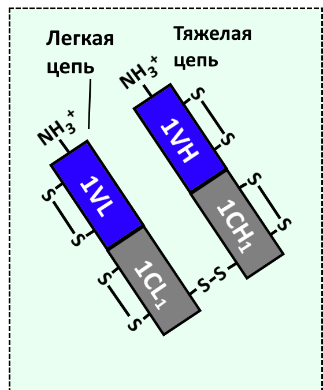
\includegraphics[width=3cm]{6} & 1 час	& 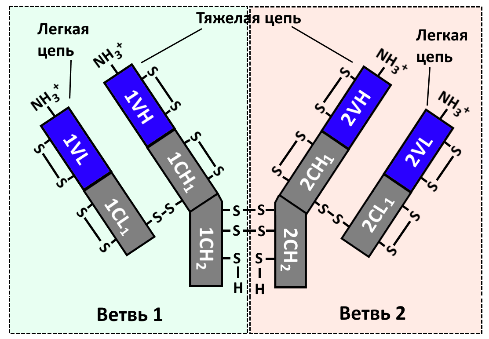
\includegraphics[width=3cm]{7} &	2 часа 30 минут \\
			\hline
			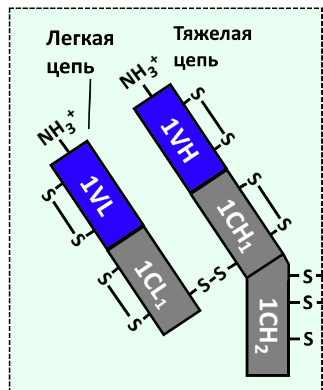
\includegraphics[width=3cm]{8} &1 час 15 минут & 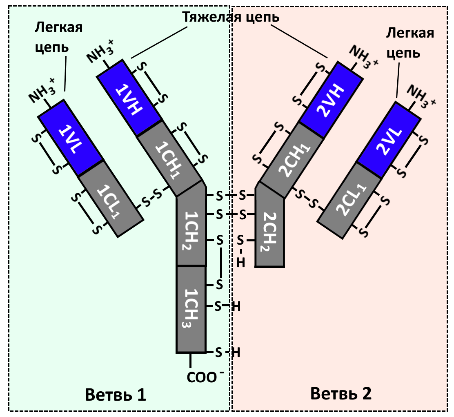
\includegraphics[width=3cm]{9} &2 часа 45 минут \\
			\hline
			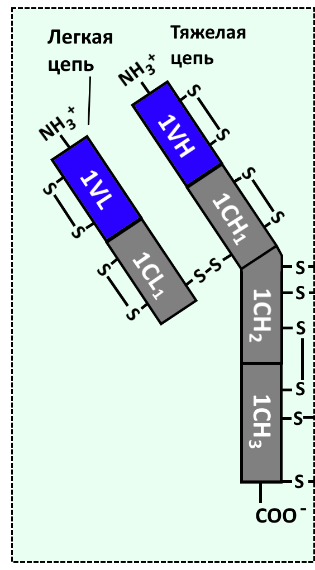
\includegraphics[width=3cm]{10} & 1 час 30 минут& 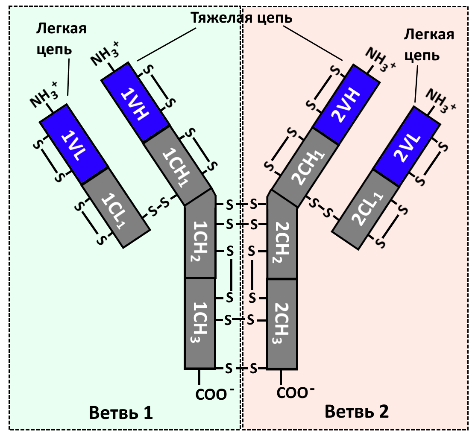
\includegraphics[width=3cm]{11} & 3 часа	\\
			\hline	
		\end{tabular}
	\end{center}
\end{table}

Каждый домен увеличивает время достижения антитела до опухоли на 15 минут

Участники при конструировании антитела указывали то, на какие мишени действуют вариабильные части (синего цвета). В случае если на одной ветви вариабильные домены разных цепей взаимодействовали с одной и той же мишенью, тогда вариабильная часть «работала». Правильные варианты выбора вариабильных доменов, а также значения селективности таких антител приведены в таблице ниже:

\markSection

Для того, чтобы победные очки начислялись за продукт (квантовые точки, дисплеи, солнечную батарею или биометки), он должен быть произведен и находиться на складе команды. В случае, если имеется большой набор одинаковых продуктов, то в турнирную таблицу попадет продукт с наивысшим качеством.

\begin{itemize}
	\item За продукт 1 уровня (квантовые точки определенного цвета), качеством 100\%, начисляется 1 победное очко. Если имеются квантовые точки разных цветов (в случае с дисплеем), то за каждый продукт будут начисляться баллы.
	\item За продукт 2 уровня, качеством 100\%, начисляется 2 победных очка.
	\item Количество победных очков понижается пропорционально качеству зачтенных продуктов.
	\item Если качество зачтенного продукта выше 90\%, за него начисляется 100\% от возможных за него баллов.
	\item Наличие на складе нескольких экземпляров одного и того же продукта не увеличивает победные очки.
	\item Также баллы начисляются за непотраченные деньги. Для этого определяется команда с максимальным количеством денег, она получает 1 балл. Остальные получают баллы пропорционально доли от максимального.
\end{itemize}

Допустим, что некоторая команда изготовила продукты 1 уровня – три цвета качеством 60\%, 80\% и 40\%. Используя эти продукты в качестве компонентов дисплеев, создала продукт 2 уровня качеством 70\%. Однако осталась неудовлетворенной полученным качеством, решила задачу повторно и создала продукт 2 уровня качеством 88\%. Засчитывается продукт наивысшего уровня (2 уровень) с наивысшим качеством (88\%). При этом у команды имелось 80000 \textpeso (известно, что максимальное количество денег, находящееся одной из команд – 120000 \textpeso).

Команда получает $1\cdot 0.6 + 1\cdot 0.8 + 1\cdot 0.4 + 2\cdot 0.88 + 80000 \textpeso /120000 \textpeso = 4.23$ победных очка.
